\chapter{Příklady virtualizace síťových funkcí}

V této kapitole budeno několik příkladů, jak lze jednoduše vytvořit NFV v prostředí OpenStack a OpenContrail pomocí heat templatu. Všechna uvedená řešení byla testována v 

\section{Heat templaty}\label{sub:interaction}



\section{LbaaS}\label{sub:interaction}

\subsection{Neutron HAproxy}\label{sub:interaction}

\subsection{AVI networks}\label{sub:interaction}

\section{FwaaS}\label{sub:interaction}

\subsection{PfSense}\label{sub:interaction}

\subsection{Fortigate VM}\label{sub:interaction}


\begin{figure}[h]
\begin{centering}
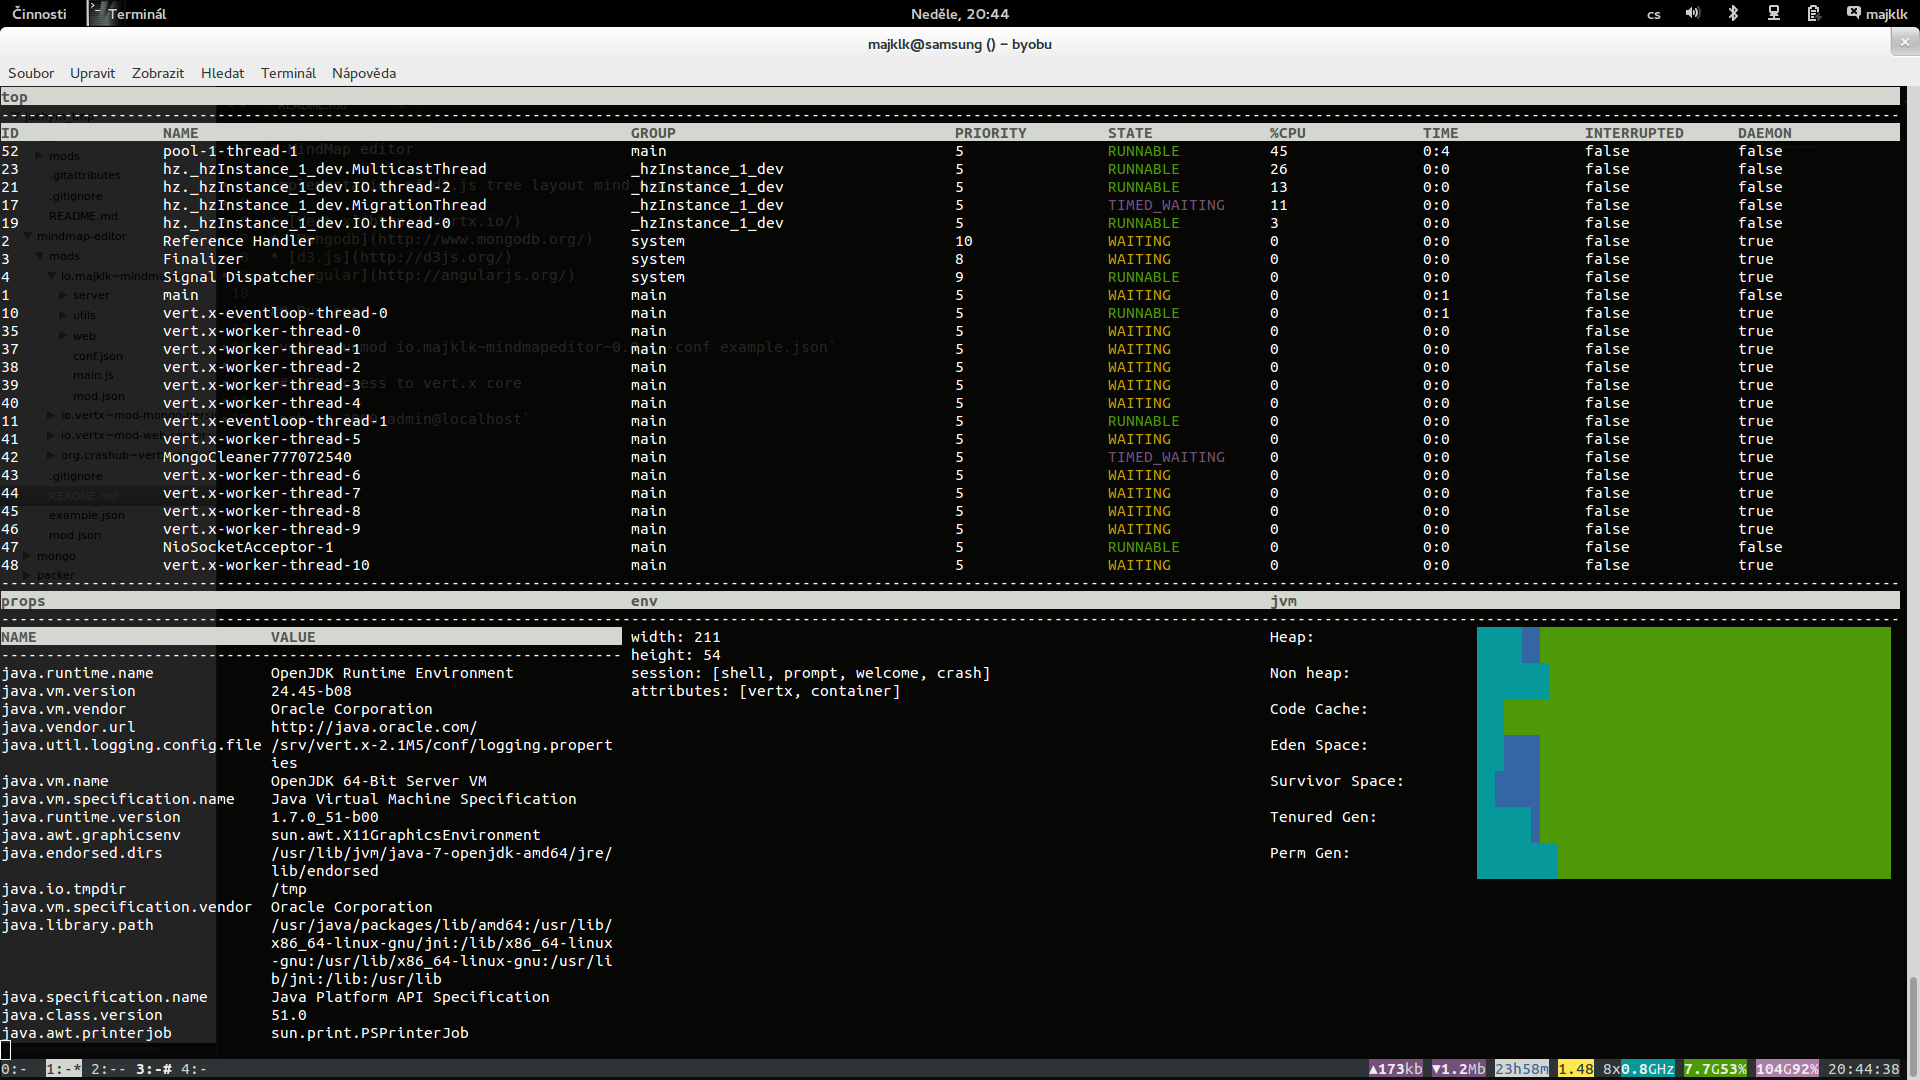
\includegraphics[scale=0.21]{images/real_interaction}
\par\end{centering}
\caption{Modul CrasHub Shell\label{fig:real_interaction}}
\end{figure}
